\documentclass[article,A4,12pt]{llncs}
\usepackage[T1]{fontenc}
\usepackage{amsmath}
\usepackage{amssymb}
\usepackage{amsfonts}
\usepackage{mathrsfs, bm}

\usepackage{graphicx}
\usepackage{tabularx}
\usepackage{subfig}
\usepackage{epsf,times}
\usepackage{color}
\usepackage{wrapfig}
\usepackage{cases}
\usepackage{multicol}

\usepackage[T1]{fontenc}
%\newcommand{\tmname}[1]{\textsc{#1}}
%\newcommand{\tmop}[1]{\ensuremath{\operatorname{#1}}}
%\newcommand{\tmsamp}[1]{\textsf{#1}}
%\newcommand{\tmtextsc}[1]{{\scshape{#1}}}
%\newcommand{\tmtextsl}[1]{{\slshape{#1}}}
%\newcommand{\tmtexttt}[1]{{\ttfamily{#1}}}

\leftmargin=0.0cm
\oddsidemargin=0.5cm
\evensidemargin=0.5cm
\topmargin=0cm
\textwidth=16.0cm
%\textheight=21.5cm
\textheight=20.0cm
\pagestyle{plain}
\setlength{\columnsep}{20pt}

\def\m{\mathbf{m}}
\def\H{\mathbf{H}}
\def\E{\mathbf{E}}
\newcommand{\vepsi}{{\varepsilon}}
\def\hnorm#1#2{\vert\,#1\,\vert_{#2}}
\newcommand{\R}{{\mathbb R}}
\newcommand{\Sph}{{\mathbb S}}
\def\x{\mathbf{x}}
\def\hvec{\overline{\mathbf{h}}}
\def\evec{\overline{\mathbf{e}}}

\newcommand{ \etal}{\mbox{\emph{et al. }}}

\newcommand\vect[1]{\mbf{#1}}
\newcommand{\mbf}[1]{\mbox{\boldmath$#1$}} 
\newcommand{\RC}[1]{#1 $\times$ #1 $\times$ #1}
\def\um{$\mu$m}
\def\C{$^{\circ}\mathrm{C}$}

\newcommand{\Rmnum}[1]{\expandafter\@slowromancap\romannumeral #1@}

% DEFINITION OF CUSTOM FONT SIZE
\newcommand{\customfontA}{\fontsize{50}{55}\selectfont}
\newcommand{\customfontB}{\fontsize{14.4}{20}\selectfont}
\newcommand{\customfontC}{\fontsize{30}{35}\selectfont}

\DeclareMathAlphabet{\mathpzc}{OT1}{pzc}{m}{it}

\def\clovek#1{\noindent\bgroup\vbox{\noindent#1}\egroup\vskip1em}

% TO INPUT BACKGROUND IMAGE
\usepackage{eso-pic}
\newcommand\BackgroundPic{
\put(0,0){
\parbox[b][\paperheight]{\paperwidth}{
\vfill
\centering
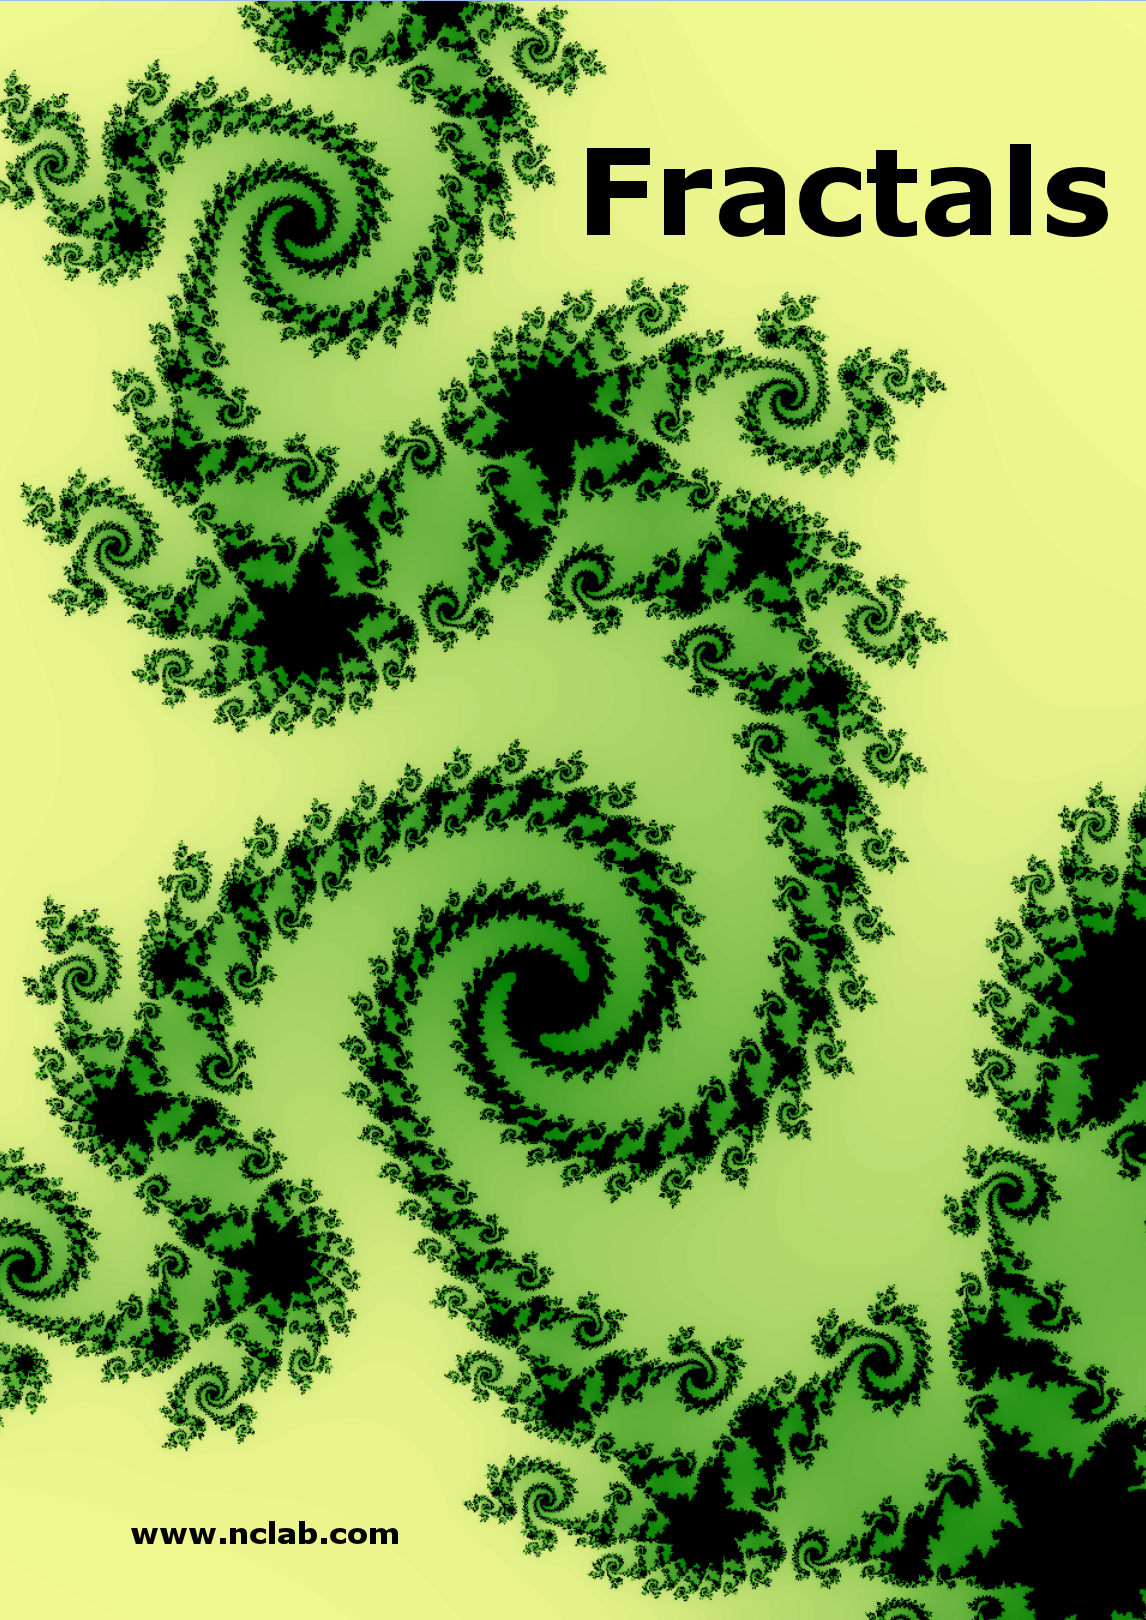
\includegraphics[width=\paperwidth,height=\paperheight]{img/julia.png}
%\includegraphics[width=\paperwidth,height=\paperheight]{img/background.jpg}
\vfill
}}}

\begin{document}

% INPUTTING BACKGROUND IMAGE
\AddToShipoutPicture{\BackgroundPic}
\vbox{}
\pagestyle{empty}
\newpage
\textwidth=15.5cm
\ClearShipoutPicture
\newpage


\section*{}
\small
\subsection*{About NCLab}
Networked Computing Laboratory (NCLab) is a popular Internet-based framework for 
programming, mathematics, computer modeling, 
and scientific computing. It serves students, instructors, researchers, and the general 
public. NCLab can be used free of charge for personal non-commercial purposes such as 
private hobby or self-education, as well as for individual non-funded academic research.
All other use is subject to {\bf purchasing a license} for a symbolic fee. The fees are as low as 
\$1 per user per month for educational use, and they are used to support the development 
and operational expenses. NCLab is a product of FEMhub Inc. The name "NCLab" is 
registered with the U.S. Patent and Trademark Office (USPTO) under Trademark No. 85420518.

\subsection*{Terms of Use and Pricing}
More details on purchasing a license and using NCLab are provided in the online documents 
{\bf Pricing} and {\bf Terms of Use} that are accessible from NCLab's home page 
{\tt http://nclab.com}.

\subsection*{Contact Information}
General inquiries: {\tt info@femhub.com}\\
Sales: {\tt sales@femhub.com}\\
NCLab support: {\tt support@nclab.com}\\
Agros \& Hermes support: {\tt support@femhub.com}\\
Web page: {\tt http://femhub.com}\\
{Physical address}\\
FEMhub Inc.\\
5490 Twin Creeks Dr.\\
Reno, NV 89523

\subsection*{About This Publication}
This publication can be copied and distributed without any restrictions
as long as reference to NCLab and FEMhub Inc. is preserved.

\subsection*{Acknowledgement}
This publication was created using freely available information about fractals
including materials from Wikipedia (http://wikipedia.org).

\normalsize

\newpage
%{\ }
%\tableofcontents
%\pagestyle{plain}

\pagestyle{plain}
\setcounter{page}{1}

\section*{Gentle Introduction to Fractals}

Prior to explaining the usage of the interactive graphical application 
Fractal Explorer in NCLab, let us briefly summarize the concept, history, 
and mathematical foundation of fractals.

\subsection*{Concept}

The word "fractal" often has different connotations for laypeople than mathematicians, where 
the layperson is more likely to be familiar with {\em fractal art} than a mathematical concept. 
The mathematical concept is difficult to formally define even for mathematicians, but key 
features can be understood with little mathematical background.

The feature of "self-similarity", for instance, is easily understood by analogy to zooming in 
with a lens or other device that zooms in on digital images to uncover finer, previously 
invisible, new structure. If this is done on fractals, however, no new detail appears; 
nothing changes and the same pattern repeats over and over, or for some fractals, nearly 
the same pattern reappears over and over. Self-similarity itself is not necessarily counter-intuitive 
(e.g., people have pondered self-similarity informally such as in the infinite regress in 
parallel mirrors or the homunculus, the little man inside the head of the little man inside 
the head...). The difference for fractals is that the pattern reproduced must be {\em detailed}.

Understanding this concept is essential for understanding fractals, so let us explain it in more 
detail. The following sequence of geometries starts with an equilateral triangle on the left.
The next geometry to the right is obtained via splitting each boundary edge of the previous 
geometry into three equally-long pieces of length $L$. Then all the middle pieces are removed, 
and always two new edges of length $L$ are added back, to add a new equilateral triangle to 
the missing middle section of each edge.\\[-6mm]

\begin{figure}[!ht]
\begin{center}
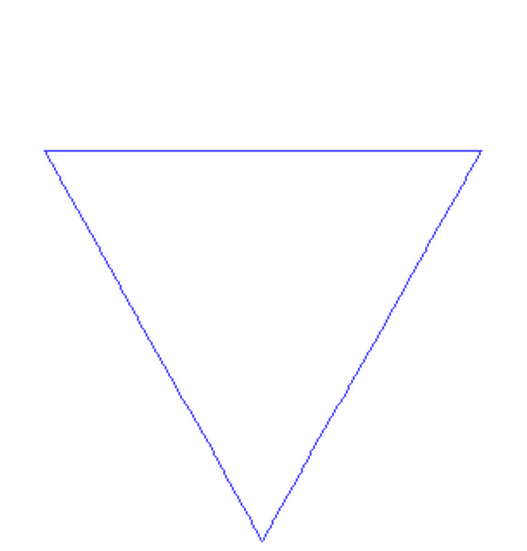
\includegraphics[width=3cm]{img/s1.png}
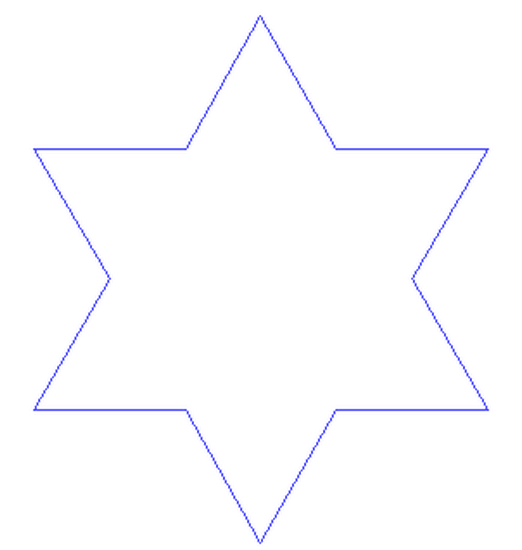
\includegraphics[width=3cm]{img/s2.png}
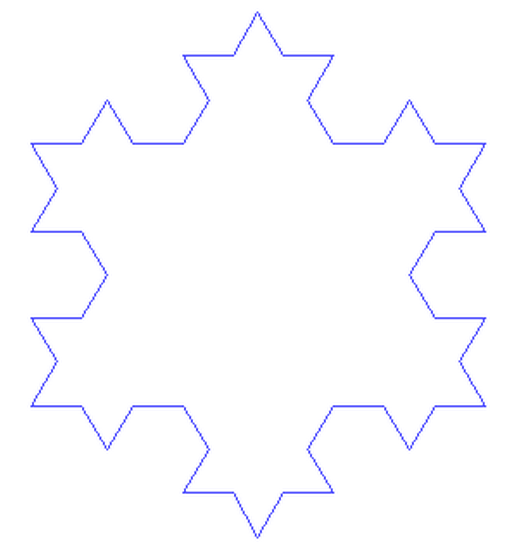
\includegraphics[width=3cm]{img/s3.png}
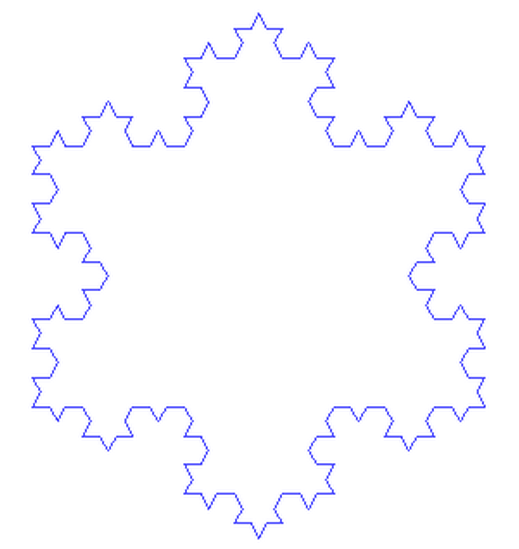
\includegraphics[width=3cm]{img/s4.png}
\end{center}
\vspace{-4mm}
\caption{First four Von Koch's curves.}
\vspace{-4mm}
\end{figure}

\noindent
Exactly the same procedure is applied to get from the second geometry to the third, and from the 
third to the fourth. These geometries are called {\em von Koch's curves} but they are not fractals 
yet. In order to get a fractal, one 
has to do this infinitely many times, and take the limit. \\

\noindent
Can you show that the boundary of the limit geometry has an infinite length?

\newpage

\noindent
This is quite interesting, given that obviously the area of the resulting fractal is finite.
It also explains that fractals 
as mathematical objects are "nowhere differentiable". In a concrete sense, this means 
fractals cannot be measured in traditional ways. To elaborate, in trying to find the length 
of a wavy non-fractal curve, one could find straight segments of some measuring tool small 
enough to lay end to end over the waves, where the pieces could get small enough to be considered 
to conform to the curve in the normal manner of measuring with a tape measure. But in measuring a 
wavy fractal curve, one would never find a small enough straight segment to conform to the curve, 
because the wavy pattern would always re-appear, albeit at a smaller size, essentially pulling 
a little more of the tape measure into the total length measured each time one attempted to 
fit it tighter and tighter to the curve. 

\subsection*{History}

The mathematical roots of the idea of fractals have been traced through a formal path of published 
works, starting in the 17th century with notions of recursion, then moving through increasingly 
rigorous mathematical treatment of the concept to the study of continuous but not differentiable 
functions in the 19th century, and on to the coining of the word fractal in the 20th century 
with a subsequent burgeoning of interest in fractals and computer-based modelling in the 21st 
century \cite{f4,f5}. The term "fractal" was first used by mathematician Benoit Mandelbrot in 
1975. Mandelbrot based it on the Latin {\em fractus} meaning "broken" or "fractured", and used 
it to extend the concept of theoretical fractional dimensions to geometric patterns in nature.

\subsection*{Mathematical Foundation}

Mathematically, a fractal is a mathematical set that has a fractal dimension that usually exceeds its topological 
dimension \cite{f1} and may fall between the integers \cite{f2}. Fractals are typically self-similar 
patterns, where self-similar means they are "the same from near as from far" \cite{f3}. Fractals may 
be exactly the same at every scale, or they may be nearly the same at different scales. The 
definition of fractal goes beyond self-similarity per se to exclude trivial self-similarity and 
include the idea of a detailed pattern repeating itself. 

Widely studied fractal sets are the Mandelbrot, Julia, and Newton sets. \\

\noindent
{\em Mandelbrot set}\\
The Mandelbrot set consists of all values 
$c$ in the complex plane for which the limit of the sequence 

$$
z_{n+1} = z_n^2 + c
$$
with the starting value $z_0 = 0$ remains bounded.\\

\noindent
{\em Julia set}\\
Let's take an arbitrary rational complex function $f(z)$ of the form  

$$
f(z) = \frac{p(z)}{q(z)}
$$
where $p(z)$ and $q(z)$ are complex polynomials.
The Julia set, usually called $J(f)$, is a set of all complex points $z_0$ 
for which the infinite sequence 

$$
z_{n+1} = f(z_n)
$$
is bounded. Currently, NCLab uses the function 

$$
f(z) = z^2 + c
$$
where $c = c_r + i c_i$ is a complex number defined using two real constants 
$c_r$ and $c_i$. More general definition of $f$ will be enabled in the future.\\

\noindent
{\em Newton set}\\
The Newton set is a special case of the Julia set, defined for an 
arbitrary non-constant complex polynomial $h(z)$ via

$$
z_{n+1} = z_n - \frac{h(z)}{h'(z)}
$$
(note that this formula corresponds to the Newton's method used
to solve nonlinear equations of the form $h(z) = 0$). In other words, the 
polynomials $p(z)$ and $q(z)$ that appear in the definition of the Julia
set are defined as

$$
p(z) = z_n h'(z) - h(z), \ \ \ \ q(z) = h'(z). 
$$
Next let us mention some basic references on fractals. The 
presentation will be continued after that with the description 
of the Fractal Explorer.


\bibliographystyle{elsarticle-num}
\begin{thebibliography}{00}

\bibitem{f0}
Wikipedia: http://wikipedia.org.

\bibitem{f1}
Mandelbrot, Benoit (2004). Fractals and Chaos. Berlin: Springer. ISBN 9780387201580. 

\bibitem{f2}
Mandelbrot,Benoit B. (1983). The fractal geometry of nature. Macmillan. ISBN 978-0-7167-1186-5. Retrieved 1 February 2012.

\bibitem{f3}
Gouyet, J-F (1996). Physics and fractal structures. Paris New York: Masson Springer. ISBN 9780387941530.

\bibitem{f4}
Edgar, Gerald (2004). Classics on Fractals. Boulder: Westview Press. ISBN 9780813341538.

\bibitem{f5}
Trochet, Holly (2009). "A History of Fractal Geometry". MacTutor History of Mathematics. Archived from the original on 4 February 2012. Retrieved 4 February 2012.

 \end{thebibliography}

%--------------------------------------------------------------------------------------
%--------------------------------------------------------------------------------------

\section*{Fractal Explorer}

The Fractal Explorer in NCLab allows the users to get familiar with the structure of the Mandelbrot
and Julia sets (Newton set is in preparation). It can be launched by clicking on the 
{\em Fractals} icon on the desktop. The following Fig. \ref{fig:man-1} shows the classical 
Mandelbrot set.\\

\begin{figure}[!ht]
\begin{center}
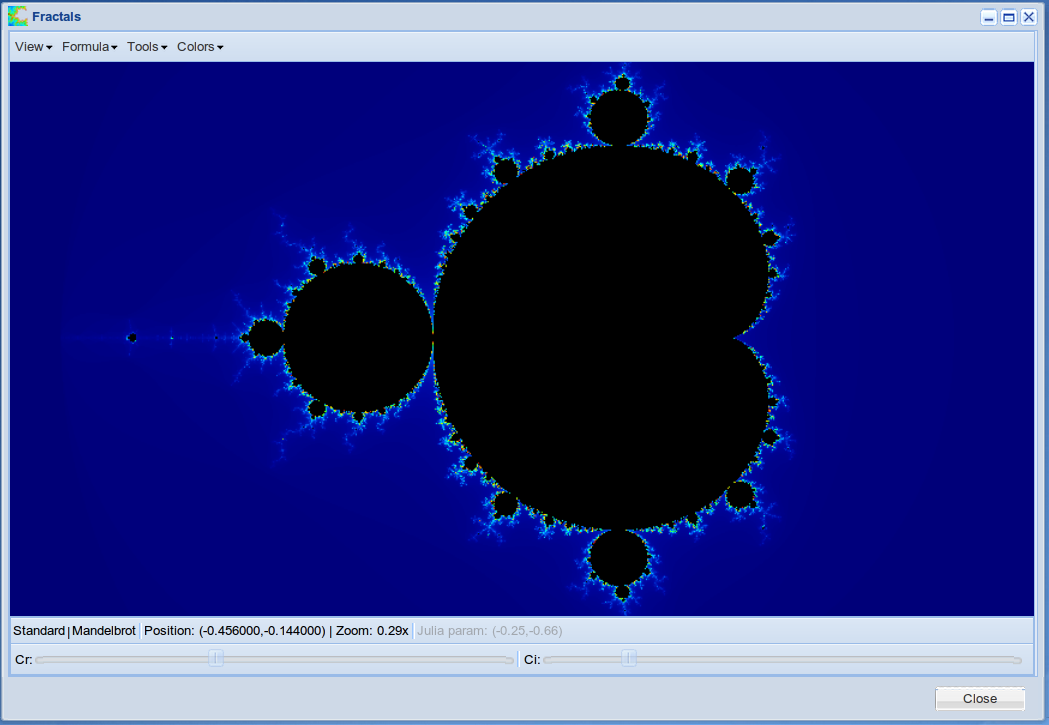
\includegraphics[width=\textwidth]{img/mandelbrot-1.png}
\end{center}
%\vspace{-2mm}
\caption{Fractal Explorer window with the Mandelbrot set.}
\label{fig:man-1}
\end{figure}

Zooming in and out is done via the mouse wheel as shown in Fig. \ref{fig:man-2}.

\clearpage

\begin{figure}[!ht]
\begin{center}
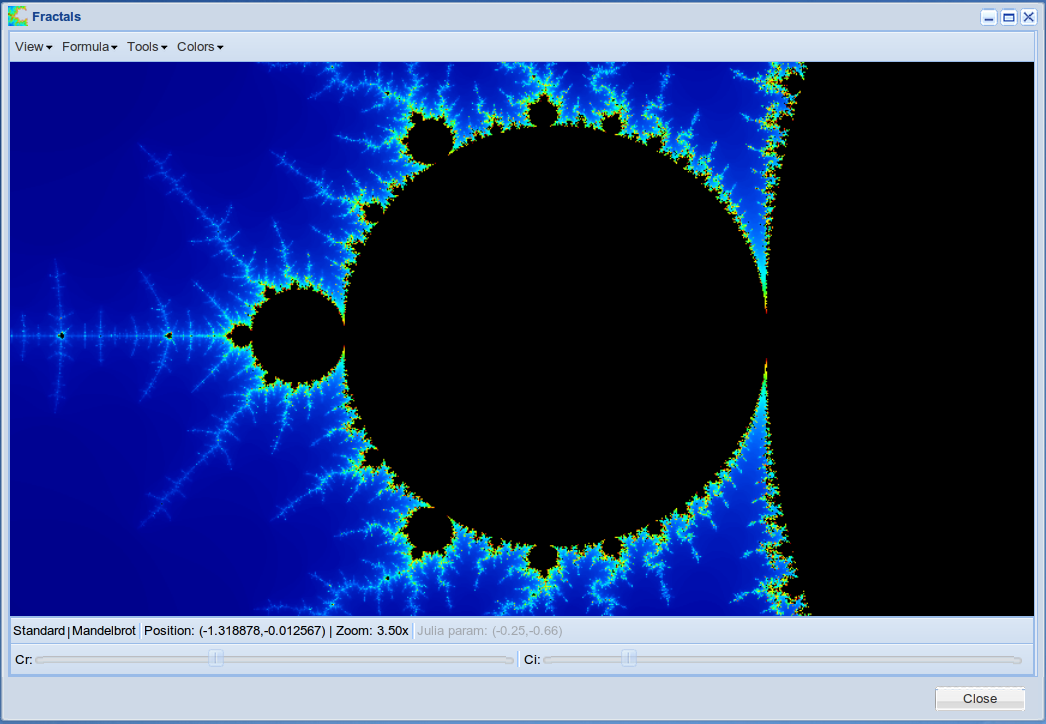
\includegraphics[width=\textwidth]{img/mandelbrot-2.png}
\end{center}
%\vspace{-2mm}
\caption{Zooming in reveals the self-similar fractal structure.}
\label{fig:man-2}
\end{figure}

\noindent
The menubar contains four items: {\em View}, {\em Formula}, {\em Tools} and {\em Colors}.

\subsection*{View Menu}
The View menu allows the user to switch between the Standard and Artistic views. When Standard view
is selected, the fractal is calculated using the standard iteration formula that was described earlier. 
With Artistic view, the Monte Carlo method is used to calculate the fractal, which has some 
interesting visual effects.

\subsection*{Formula Menu}

Here the user can select between the Mandelbrot and Julia sets. If the latter is selected, two
sliders in the bottom part of the window are activated, as shown in 
Fig. \ref{fig:jul-1}.

\clearpage

\begin{figure}[!ht]
\begin{center}
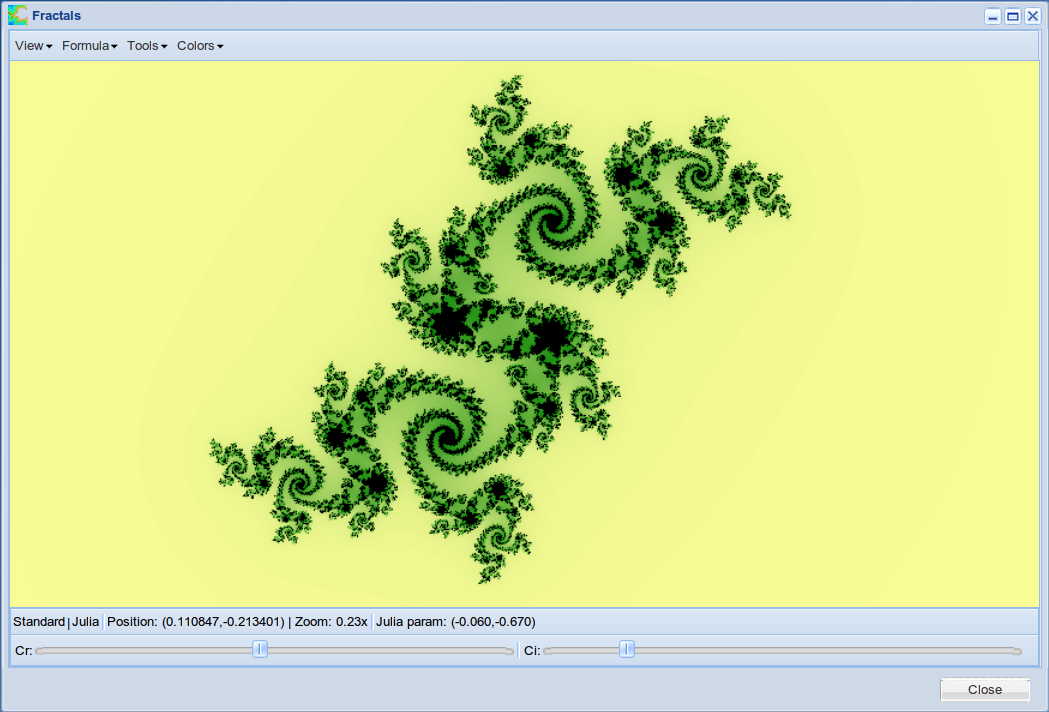
\includegraphics[width=\textwidth]{img/julia-1.png}
\end{center}
%\vspace{-2mm}
\caption{Sample Julia fractal. Constants $c_r$ and $c_i$ can be adjusted using sliders.}
\label{fig:jul-1}
\end{figure}

\noindent
The sliders represent the real and imaginary parts $c_r, c_i$ of the complex constant 
$c = c_r + i c_i$ in the formula $f(z) = z^2 + c$. When they are moved, the Julia 
fractal changes instantly. Of course not all values of the Julia constants are 
available through the sliders. This brings us to the {\em Tools} menu.

\subsection*{Tools Menu}

This menu can be used to

\begin{itemize} 
\item Change the center and zoom of the fractal view. 
\item Set the constants $c_r$ and $c_i$ manually.
\item Reset the center and zoom to initial values.
\end{itemize}

\subsection*{Colors Menu}

In the Colors menu one can choose between the default palette and a wide
range of linear gradients. Fig. \ref{fig:lingrad} shows the linear gradient 
menu.

\begin{figure}[!ht]
\begin{center}
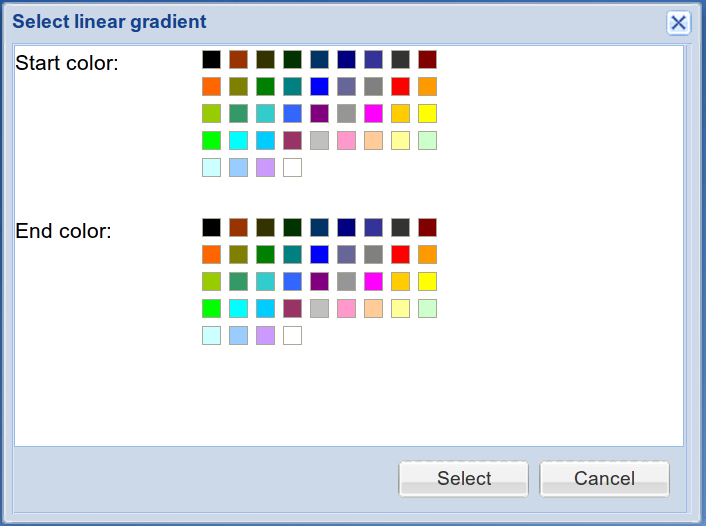
\includegraphics[width=0.6\textwidth]{img/lingrad.png}
\end{center}
%\vspace{-2mm}
\caption{Color menu for linear gradients.}
\label{fig:lingrad}
\end{figure}

\noindent
The start and end colors for the linear interpolation are selected
by clicking on one color in the upper part and one color in the lower 
part, respectively. After pressing Select, the linear gradient is 
applied.



\end{document}
